\chapter{初探微积分}

\section{高等数学之门---抛物线下的面积与微积分}

\begin{figure}
  \centering
    \documentclass[border=3pt]{standalone}
\usepackage{tikz}
\usepackage{amsmath}
\usepackage{amssymb}
\usepackage{ctex}
\usetikzlibrary{matrix, calc, positioning}
\usepackage{pgfplots}
\pgfplotsset{compat=1.18}

\begin{document}

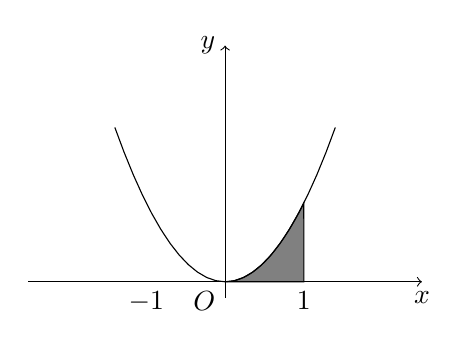
\begin{tikzpicture}
	\draw[->](-2.5,0)--(2.5,0)node[below]{$x$};
	\draw[->](0,-0.2)--(0,3)node[left]{$y$};
	\node[below left]at(0,0){$O$};
	\draw[fill=gray,domain=0:1] (0,0) -- plot({\x},{(\x)^2}) -- (1,0) -- cycle;
	\draw[domain=-1.4:1.4] plot({\x}, {(\x)^2});
	\node[below]at(1,0){$1$};
	\node[below]at(-1,0){$-1$};
\end{tikzpicture}

\end{document}

  \caption{square}\label{fig:square}
\end{figure}

如\cref{fig:square}, 对于这样的抛物线, 大家最熟悉不过了, 但如图所示的阴影面积怎么求呢?
自古希腊人发现抛物线以后, 这个问题长时间困扰着数学家们.
直到微积分的发明才使这个问题有了系统的解法.

先看不用微积分的解法:
我们先给出一个公式:

\[
  1^{2}+2^{2}+3^{2}+\ldots + n^{2} = \frac{n(n+1)(2n+1)}{6}
.\]

\begin{proof}
  对于数列 $\{a_{n}\} $, $a_n = (n+1)^{3}- n ^{3} = 3n^{2}+3n+1$
  \begin{align}
    \sum_{i=1}^{n} a_n & = (n+1)^{3}-1                                     \\
    & = 3 \sum_{i=1}^{n} i^{2} + 3 \sum_{i=1}^{n} i + n
  \end{align}
  \begin{equation*}
    \sum_{i=1}^{n} i^{2} = \frac{1}{3} \left[(n+1)^{3} -n -1 \right]
    - \frac{n(n+1)}{2}  = \frac{n(n+1)(2n+1)}{6}
  \end{equation*}
\end{proof}

\begin{figure}
  \centering
    \documentclass[border=3pt]{standalone}
\usepackage{tikz}
\usepackage{amsmath}
\usepackage{amssymb}
\usepackage{ctex}
\usetikzlibrary{matrix, calc, positioning}
\usepackage{pgfplots}
\pgfplotsset{compat=1.18}

\begin{document}
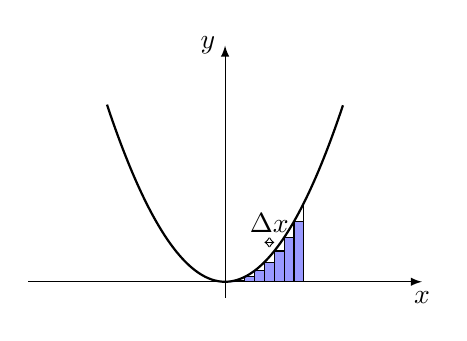
\begin{tikzpicture}[declare function={f(\x)=(\x)^(2);},
		lnode/.style={fill=white,font=\small,inner sep=0pt}]
	\newcommand*{\N}{8}
	\pgfmathtruncatemacro{\M}{\N/4}
	\coordinate (start) at (0,{f(0)});
	\foreach \X [remember=\X as \LastX (initially 0)] in {1,...,\N}
		{
			\draw[fill=blue!40!white] (\LastX/\N,0) rectangle (\X/\N,{f(\LastX/\N)});
			% \draw[red,fill=red] (1+\LastX*4/\N,{f(1+\LastX*4/\N)}) circle (2pt) ;
			\path  (\LastX/\N,0pt) coordinate (x\X);
		}
	\coordinate (end) at (1,{f(1)});
	\draw (1,0)--(1,{f(1)});
	\draw [-latex] (-2.5,0) -- (2.5,0) node (xaxis) [below] {$x$};
	\draw [-latex] (0,-0.2) -- (0,3) node [left] {$y$};
	\draw[domain=-1.5:1.5,samples=200,variable=\x,-,thick] plot ({\x},{f(\x)});
	\draw[<->] (x5|- 0,1/2)--(x6|- 0,1/2) node[above, midway] {$\Delta x$};
\end{tikzpicture}

\end{document}

  \caption{矩形逼近} \label{fig:rect}
\end{figure}

下面回归正题,
如 \cref{fig:rect}, 我们把 $y=x^{2} $ 中 $[0, 1]$ 部分分成$n$个矩形,
每条矩形的底边为 $ \frac{1}{n} = \Delta x $.

对于第$i$个矩形, 由于其前方有$i-1$个矩形,
故其高为 $h_i = f(i \Delta x) = \frac{i^{2}}{n^{2} } $.
这$n$个矩形的面积和为
\begin{align*}
  S & = \sum_{i=1}^{n} \Delta x \cdot h_i  \\
  & = \frac{1}{n^3} \sum_{i=1}^{n} i^{2} \\
  & = \frac{n(n+1)(2n+1)}{6n^3 }
\end{align*}

当$n \to +\infty$时,
这$n$个矩形的面积和可近似认为是 $f(x) = y = x^{2},x\in [0, 1] $ 与X轴围成的面积.
而
\[
  \lim_{n \to \infty} \frac{n(n+1)(2n+1)}{6n^3 } = \frac{1}{3}
.\]

故面积$ S = \frac{1}{3}$.

但这样做法十分麻烦, 况且如果不是二次函数, 在矩形面积求和时, 便会遇到障碍.
若此题用积分做, 则有
\[
  \int_{0}^{1} x^{2} \dif x= \frac{1}{3}
.\]
\begin{definition}[积分]
  若 $F'(x) = f(x)$, 则 $\int f(x) \dif x = F(x)$, 其中 「$\int $」 为积分号,
  $f(x)$称为被积函数, 「$\dif x$」称为微分算子, $F(x)$称为原函数.
\end{definition}
显然积分是求导的逆运算.

由导数的运算法则, 不难看出积分有以下法则:
\begin{enumerate}

  \item \label{law1} 若 $\int f(x) \dif x = F(x)$, 则 $\int  f(x) \dif x
    = F(x) + C$. $C = \mathrm{Constant} $(任意常数).
  \item $\int [f(x) \pm g(x)] \dif x = \int f(x) \dif x \pm \int g(x) \dif x$
  \item $\int \lambda f(x) \dif x = \lambda \int f(x) \dif x$,
    其中$\lambda $为任意常数.

\end{enumerate}

注意由\cref{law1} 法则可以知道, 一个函数有无数个原函数,
但任意两个函数之差为常数.

且对于形如 $\int f(x)g(x) \dif x,\quad \int \frac{f(x)}{g(x)} \dif x$ 这样的积分无法直接计算.

下面我们来计算一些函数的积分:
\begin{align*}
  \int x^{2} \dif x  & = \frac{1}{3} x ^3 +C \\
  \int \cos x \dif x & = \sin x + C
\end{align*}

事实上, 像导数表一样, 积分的运算也有积分表.

\[
	\int k \, \dif x           = kx + C
	.\]
\[
	\int x^n \, \dif x         = \frac{x^{n+1}}{n+1} + C \quad (n \neq -1)
	.\]
\[
	\int \frac{1}{x} \, \dif x = \ln|x| + C
	.\]
\[
	\int e^x \, \dif x         = e^x + C
	.\]
\[
	\int a^x \, \dif x         = \frac{a^x}{\ln a} + C \quad (a > 0, a \neq 1)
	.\]
\[
	\int \sin x \, \dif x      = -\cos x + C
	.\]
\[
	\int \cos x \, \dif x      = \sin x + C
	.\]
\[
	\int \tan x \, \dif x      = -\ln|\cos x| + C
	.\]


上述公式的证明, 由 求导法则 易证.

看到这里你可能会疑惑, 为什么要用$\int \,\dif x$这两个符号表示积分呢?
下面介绍另一个概念---微分.

\begin{figure}[ht]
  \centering
    \documentclass[border=3pt,tikz]{standalone}
\usepackage{tikz}
\usepackage{amsmath}
\usepackage{amssymb}
\usepackage{ctex}
\usetikzlibrary{matrix, calc, positioning}
\begin{document}
\providecommand*{\N}{6}
\renewcommand*{\N}{6}
\begin{tikzpicture}[scale=1.2,declare function={f(\x)=((0.12)*(\x)^(3)-0.9*(\x)^(2)+2.2*\x+0.8;},
		lnode/.style={fill=white,font=\normalsize,inner sep=0pt,text height=1.5em}]
	\pgfmathtruncatemacro{\M}{\N/4}
	\coordinate (start) at (.8,{f(.8)});
	\coordinate (end) at (5.05,{f(5.05)});
	\draw (4,{f(4)})--(5,{f(4)}) node[below,midway, lnode] {$\mathrm{d} x$};
	\draw (5,{f(4)})--(5,{f(5)}) node[right, midway] {$\mathrm{d} y$};
	\draw (4,{f(4)})--(5,{f(5)}) ;
	\draw [-latex] (-0.5,0) -- (6,0) node (xaxis) [below] {$x$};
	\draw [-latex] (0,-0.5) -- (0,5) node [left] {$y$};
	\draw[domain=0.5:5.2,samples=200,variable=\x,-,thick] plot ({\x},{f(\x)});
	% \draw[<->] (x2|- 0,{f(\x)-1/2})--(x3|- 0,{f(\x)-1/2}) node[above,midway] {$\Delta x$};
\end{tikzpicture}
\end{document}

    \caption{微分近似}\label{fig:simdx}
\end{figure}

由\cref{fig:simdx}, 当 $\Delta x \to 0$时,
我们记 $\Delta y = f(x+\Delta x) - f(x)$为$f(x)$在点$x$处的微分.
此时我们记$\dif y = \dif f(x) = \lim_{\Delta x \to 0} \Delta y $, $\dif x
= \lim_{\Delta x\to 0} \Delta x$,
由导数的定义式, 我们有
\begin{align}
  \frac{\dif y}{\dif x} & = \frac{f(x+\dif x) - f(x)}{\dif x} = f'(x)
  \label{eqn:directive}                                               \\
  \dif y                & = f'(x) \dif x \label{eqn:dydx}
\end{align}

\begin{note}[微分近似] \label{note:simdx}
  注意\cref{fig:simdx}, 从几何意义上来理解, 这里的$\dif y = f'(x) \dif x $就是说,
  当一个曲线上两点间距离足够近时, 我们可以用这一点的切线的变化量
  $f'(x) \dif x $去近似这条曲线的变化量 $\dif y$.
\end{note}

基于\cref{eqn:directive,eqn:dydx}, 我们可以知道微分的运算法则
\begin{align}
  \dif C                           & = 0
  \\
  \dif [ \lambda f(x) + \mu g(x) ] & = \lambda f'(x) \dif x + \mu
  g'(x) \dif x \label{eqn:linearity}                                \\
  \dif f(x)                        & = \dif [f(x)+C] = f'(x) \dif x
\end{align}

结合前面积分的定义, 对于$F'(x) = f(x)$ 有,
\[
  \int f(x) \dif x = F(x) + C
.\]
又有
\[
  f(x) \dif x = \dif[F(x) +C]
.\]
于是
\[
  \int \dif [F(x) +C] = F(x)+C
.\]

从中可以看出 $\int \text{与} \dif $连用可以相互抵消
\footnote{
  编者注:$\Delta x \to 0$ 时记为$\dif x$,
  历史上$\int $其实是$\sum_{i}^{\infty}$的简写(因为它写起来太麻烦了).
  从几何意义上来理解,
  $\int f(x) \dif x = \lim_{\Delta x \to 0} \sum_{i}^{\infty} f'(x_i)
  \cdot \Delta x_i$
  就是将每一点$x_i$函数的增量$\Delta y$都用 \cref{note:simdx}中提到的微分近似去替代,
  无限段增量累加, 便是原函数的变化量. 这也可以从几何上解释\emph{牛顿--莱布尼兹定理}.
},
即积分是微分的逆运算.

下面请读者利用以上知识证明以下等式:
\begin{align}
  \int \dif f(x)                              & = f(x)+C
  \\
  \int f(x) \dif g(x)                         & = \int f(x)g'(x) \dif
  x                                                                   \\
  \int  f(x) \dif g(x) + \int  g(x) \dif f(x) & = f(x) \cdot g(x) +C
  \label{eqn:fxgx'}
\end{align}

讲了这么多, 这和计算抛物线下面积有什么关系呢?
事实上, 我们有如下的\textbf{牛顿--莱布尼兹定理}.

\begin{theorem}[牛顿--莱布尼兹定理]
  对于 $F'(x) = f(x)$,
  \[
    \int _{a} ^{b} f(x) \dif x = F(b) - F(a)
  .\]
\end{theorem}

(编者注:从几何意义上来说)$\int _a^b f(x) \dif x$ 表示 $f(x)$在 $[a,b]$上与$x$轴围成的\emph{有向面积}
\footnote{编者注:这里「有向」二字为编者补充, $b>a>0,\And f(x)>0$ 时, $I = \int _a ^b
  f(x) \dif x >0$,
其中积分号下方的$a$称为\emph{积分下限}, 积分号上方$b$称为\emph{积分上限}, 交换积分上下限, 结果为$-I$}.

当 $f(x)$ 在 $[a,b]$ 上$>0$ 时, $\int _a ^{b} f(x) \dif x $为正值.
当 $f(x)$ 在 $[a,b]$ 上$<0$ 时, $\int _a ^{b} f(x) \dif x $为负值.

下面我们来证明$f(x)> 0,x \in [a,b]$的情形.

\begin{figure}[htbp]
  \centering
    \documentclass[border=3pt,tikz]{standalone}
\usepackage{tikz}
\usepackage{amsmath}
\usepackage{amssymb}
\usepackage{ctex}
\usetikzlibrary{matrix, calc, positioning}
\begin{document}
\providecommand*{\N}{6}
\renewcommand*{\N}{6}
\begin{tikzpicture}[scale=1.2,declare function={f(\x)=((0.12)*(\x)^(3)-0.93*(\x)^(2)+1.6*\x+2.3;},
		lnode/.style={fill=white,font=\normalsize,inner sep=0pt,text height=1.5em}]
	\pgfmathtruncatemacro{\M}{\N/4}
	\coordinate (start) at (.8,{f(.8)});
	\foreach \X [remember=\X as \LastX (initially 0)] in {1,...,\N}
	{\draw[fill=orange!40!white] (1+\LastX*4/\N,0) rectangle (1+\X*4/\N,{f(1+\LastX*4/\N)});
	% \draw[red,fill=red] (1+\LastX*4/\N,{f(1+\LastX*4/\N)}) circle (2pt) ;
	\path  (1+\LastX*4/\N,0pt) coordinate (x\X);
	\ifnum\X=1
		\draw (1+\LastX*4/\N,3pt) -- (1+\LastX*4/\N,0pt) coordinate (x\X)
		node[anchor=north east,xshift=2pt,lnode]  {$a=x_{\X}$};
	\else
		\pgfmathtruncatemacro{\itest}{mod(\X,\M)}
		\ifnum\itest=0
			\pgfmathsetmacro{\dist}{4-\LastX*4/\N}
			\ifdim\dist cm>5pt
				\draw (1+\LastX*4/\N,3pt) -- (1+\LastX*4/\N,0pt)
				node[anchor=north,lnode] {$x_{\X}$};
			\fi
		\fi
	\fi
	}
	\coordinate (end) at (5.05,{f(5.05)});
	\draw (5,3pt) -- (5,0pt)
	node[anchor=north west,xshift=-2pt,lnode]{$b=x_n$};
	\draw (5,0)--(5,{f(5)});
	\draw [-latex] (-0.5,0) -- (6,0) node (xaxis) [below] {$x$};
	\draw [-latex] (0,-0.5) -- (0,5) node [left] {$y$};
	\draw[domain=0.5:5.2,samples=200,variable=\x,red,-,thick] plot ({\x},{f(\x)});
	\draw[<->] (x2|- 0,-1)--(x3|- 0,-1) node[above,midway] {$\Delta x$};
\end{tikzpicture}
\end{document}

  \caption{a到b的矩形逼近}\label{fig:absim}
\end{figure}

如\cref{fig:absim}, 把这个不规则图形分为$n$个矩形,
每个矩形的底 $\dif x = x_n - x_{n-1} =\frac{b-a}{n}$,
对于第$i$个矩形, 其高

\begin{align*}
  h_i & = f(a+ i \cdot \frac{b-a}{n}) \\
  & = f(a+ i \dif x)
\end{align*}

\begin{align*}
  S_i & = \dif x \cdot f(a+i \dif x)         \\
  & = \dif F(a+i\dif x)                  \\
  & = F(a+ i \dif x) - F(a+(i-1) \dif x)
\end{align*}

总面积

\begin{align*}
  \sum_{i=1}^{\infty} S_i  = F(a+\dif x ) - F(a) + F(a+2 \dif x -
  F(a+\dif x )) +\ldots \\
  + F(a+n\dif x) - F(a+ (n-1)\dif x)
  \notag                \\
  = F(a+n \dif x) - F(a)
\end{align*}

又因为
\[
  n\dif x = b-a
.\]
故
\[
  \sum_{i=1}^{\infty} S_i = \int _a^{b} f(x) \dif x = F(b) - F(a)
.\]
小于零的情况同理, 至于积分的一般方法与应用请见下一节.

\paragraph{注}
这里对积分的讨论是相对粗略的极不严谨的, 对于微积分如果要严谨讨论,
我们需要讨论极限的存在准则,
实数集的完备性, 函数的两类间断点, 连续性, 可导性, 可积性以及$\epsilon \text{-} \delta $语言等.
感兴趣的同学可以自行查阅资料, 这里限于篇幅无法详细解读.

\section{积分技巧及微积分的应用}
上一节我们介绍了微积分的一些基本概念. 现在我们来讲积分的技巧及应用.

\subsection{积分技巧}
请熟知 \cref{eqn:fxgx'}.
\subsubsection*{换元法}
换元法分两类, 一类是令$x = \varphi (t)$使得$\int f(x)\dif x $转化为$\int
f\left[\varphi (t)\right] \cdot \varphi '(t) \dif t$的形式,
最后再令 $t = \varphi ^{-1} (x) $.
另一类换元法是令$t=\Phi (x)$, 转化与前者类似, 最后将结果中的$t$代换成$\Phi (x)$.

不管哪种方法, 其核心是找到一个与$x$相关的变量$t$, 对$t$进行积分, 再将$x$代回结果中.

\begin{example}
  \[
    I = \int \sqrt{1-x^{2} } \dif x, 0 \leq x \leq 1
  .\]

  它的原函数我们注意力不够, 看不出来.

  不妨令$x = \cos t,t \in \left[0,\frac{\pi}{2} \right]$
  则原积分
  \begin{align*}
    I & = \int  \sin t \dif \cos t                        \\
    & = - \int \sin ^{2} t \dif t                       \\
    & = \int \frac{ \cos 2t }{2} \dif t - \frac{1}{2} t
  \end{align*}

  再令$\mu  = 2t$, 则
  \begin{align*}
    \int \frac{\cos 2t}{2}\dif t & = \int \frac{\cos  \mu}{2} \dif
    \frac{\mu}{2}                                                       \\
    & = \frac{1}{4} \int \cos \mu \dif \mu \\
    & = \frac{1}{4} \sin \mu               \\
    & = \frac{1}{4} \sin  2t + C
  \end{align*}

  故原积分
  \begin{align*}
    I & = \frac{1}{4} \sin  2t - \frac{1}{2}t +C                    \\
    & = \frac{1}{4} \sin 2(\arccos x ) - \frac{1}{2} \arccos x +C
  \end{align*}
  其中$\arccos x$表示$\cos x$的反函数.
\end{example}

\subsubsection*{分部积分法}
由恒等式
\[
  \int f(x)\dif g(x) + \int g(x) \dif f(x) = f(x)\cdot g(x)
.\]
可以导出以下积分技巧:
对于$\int f(x)g(x) \dif x$型积分, 令$F'(x) = f(x)$, $G'(x) = g(x)$, 则
\begin{align*}
  \int f(x)g(x) \dif x & = G(x)f(x) - \int G(x) \dif f(x) \\
  & = F(x)g(x) - \int F(x) \dif g(x)
\end{align*}
两个等式, 哪个方便用哪个.

\begin{example}
  \begin{align*}
    \int x \sin x\dif x & = - \int x \dif \cos x                          \\
    & = -\left(x \cos x - \int  \cos x \dif x \right) \\
    & = \sin x - x \cos x +C
  \end{align*}
\end{example}
别忘了, $\int \dif$  的常数可以直接提出来, 参见 \cref{eqn:linearity}.

\subsection{积分的应用}
本节主要涉及定积分, 若一个函数的不定积分可求, 则其求定积分易如反掌.

\subsubsection{圆锥体积推导}

如 \cref{fig:circular_cone}, 高$PO = h$, 底面积$S$, 在$PO$上取一点$M$,
作平行于底面的截面$\odot M$, 记$PM = x$, 则
\[
  S_m = \frac{x^{2}}{h^{2} } \cdot S
.\]

过点$M$ 作一段无穷小的高$\dif x$.
则
\[
  \frac{x^{2}}{h^{2} }\cdot S \cdot \dif x = \dif V
.\]

\begin{figure}[htbp]
  \centering
    \begin{subfigure}{0.45\textwidth}
      \centering
      \documentclass[12pt,tikz]{standalone}
\usepackage{xcolor}
\usepackage{tikz}
\usepackage{tikz-3dplot}

\begin{document}
\pgfmathsetmacro\th{65}
\pgfmathsetmacro\az{110}
\tdplotsetmaincoords{\th}{\az}
%parameters of the cone
\begin{tikzpicture}[scale=1, tdplot_main_coords, axis/.style={blue,thick}]
	\pgfmathsetmacro\R{2} %radius of base
	\pgfmathsetmacro\v{5} %height of cone
	\pgfmathsetmacro\M{3}
	\path (0,0,0) coordinate (O)
	(0,0,\M) coordinate (M)
	(0,0,\v) coordinate (P);
	\foreach \point/\pos in {P/above, O/below, M/left}
		{\fill (\point) circle[radius=1pt] node[\pos] {$\point$};}
	\draw[dashed] (P) -- (O);

	\pgfmathsetmacro\RM{\R - \M*\R/\v}

	\pgfmathsetmacro\cott{{cot(\th)}}
	\pgfmathsetmacro\fraction{\R*\cott/\v}
	\pgfmathsetmacro\fraction{\fraction<1 ? \fraction : 1}
	\pgfmathsetmacro\angle{{acos(\fraction)}}

	% % angles for transformed lines
	\pgfmathsetmacro\PhiOne{180+(\az-90)+\angle}
	\pgfmathsetmacro\PhiTwo{180+(\az-90)-\angle}

	% % coordinates for transformed surface lines
	\pgfmathsetmacro\sinPhiOne{{sin(\PhiOne)}}
	\pgfmathsetmacro\cosPhiOne{{cos(\PhiOne)}}
	\pgfmathsetmacro\sinPhiTwo{{sin(\PhiTwo)}}
	\pgfmathsetmacro\cosPhiTwo{{cos(\PhiTwo)}}

	\tdplotdrawarc[tdplot_main_coords,dashed]{(O)}{\R}{\PhiTwo}{\PhiOne}{anchor=north}{}
	\tdplotdrawarc[tdplot_main_coords,thick]{(O)}{\R}{\PhiOne}{360+\PhiTwo}{anchor=north}{}

	\tdplotdrawarc[tdplot_main_coords,dashed]{(M)}{\RM}{\PhiTwo}{\PhiOne}{anchor=north}{}
	\tdplotdrawarc[tdplot_main_coords,thick]{(M)}{\RM}{\PhiOne}{360+\PhiTwo}{anchor=north}{}

	% % displaying transformed surface of the cone (rotated)
	\draw[thick] (0,0,\v) -- (\R*\cosPhiOne,\R*\sinPhiOne,0);
	\draw[thick] (0,0,\v) -- (\R*\cosPhiTwo,\R*\sinPhiTwo,0);
\end{tikzpicture}
\end{document}

      \caption{$M$点截面}\label{fig:circular_cone}
    \end{subfigure}
    \begin{subfigure}{0.45\textwidth}
      \centering
      \documentclass[12pt,tikz]{standalone}
\usepackage{xcolor}
\usepackage{tikz}
\usepackage{tikz-3dplot}

\begin{document}
\pgfmathsetmacro\th{65}
\pgfmathsetmacro\az{110}
\tdplotsetmaincoords{\th}{\az}
%parameters of the cone
\begin{tikzpicture}[scale=1, tdplot_main_coords, axis/.style={blue,thick}]
	\pgfmathsetmacro\R{2} %radius of base
	\pgfmathsetmacro\v{5} %height of cone
	\pgfmathsetmacro\M{3}
	\path (0,0,0) coordinate (O)
	(0,0,\M) coordinate (M)
	(0,0,\v) coordinate (P);
	\foreach \point/\pos in {P/above, O/below, M/left}
		{\fill (\point) circle[radius=1pt] node[\pos] {$\point$};}
	\draw[dashed] (P) -- (O);

	\pgfmathsetmacro\RM{\R - \M*\R/\v}

	% \draw[thick,->] (0,0,0) -- (1,0,0) node[anchor=north east]{$x$};
	% \draw[thick,->] (0,0,0) -- (0,1,0) node[anchor=north west]{$y$};
	% \draw[thick,->] (0,0,0) -- (0,0,1) node[anchor=south]{$z$};

	\pgfmathsetmacro\cott{{cot(\th)}}
	\pgfmathsetmacro\fraction{\R*\cott/\v}
	\pgfmathsetmacro\fraction{\fraction<1 ? \fraction : 1}
	\pgfmathsetmacro\angle{{acos(\fraction)}}

	% % angles for transformed lines
	\pgfmathsetmacro\PhiOne{180+(\az-90)+\angle}
	\pgfmathsetmacro\PhiTwo{180+(\az-90)-\angle}

	% % coordinates for transformed surface lines
	\pgfmathsetmacro\sinPhiOne{{sin(\PhiOne)}}
	\pgfmathsetmacro\cosPhiOne{{cos(\PhiOne)}}
	\pgfmathsetmacro\sinPhiTwo{{sin(\PhiTwo)}}
	\pgfmathsetmacro\cosPhiTwo{{cos(\PhiTwo)}}

	\tdplotdrawarc[tdplot_main_coords,dashed]{(O)}{\R}{\PhiTwo}{\PhiOne}{anchor=north}{}
	\tdplotdrawarc[tdplot_main_coords,thick]{(O)}{\R}{\PhiOne}{360+\PhiTwo}{anchor=north}{}

	\tdplotdrawarc[tdplot_main_coords,dashed]{(M)}{\RM}{\PhiTwo}{\PhiOne}{anchor=north}{}
	\tdplotdrawarc[tdplot_main_coords,thick]{(M)}{\RM}{\PhiOne}{360+\PhiTwo}{anchor=north}{}

	% % displaying transformed surface of the cone (rotated)
	\draw[thick] (0,0,\v) -- (\R*\cosPhiOne,\R*\sinPhiOne,0);
	\draw[thick] (0,0,\v) -- (\R*\cosPhiTwo,\R*\sinPhiTwo,0);
	\pgfmathsetmacro\N{1}

	\foreach \X [remember=\X as \LastX (initially 0)] in {0, \N,...,\v}
		{
			\path (0,0,\X) coordinate (X);
			\path (0,0,\LastX) coordinate (L);
			\pgfmathsetmacro\RX{\R - \X*\R/\v}
			\pgfmathsetmacro\RLX{\R - \LastX*\R/\v}

			\tdplotdrawarc[tdplot_main_coords]{(X)}{\RX}{\PhiOne}{360+\PhiTwo}{anchor=north}{};
			\tdplotdrawarc[tdplot_main_coords]{(L)}{\RX}{\PhiOne}{360+\PhiTwo}{anchor=north}{};

			\tdplotdrawarc[tdplot_main_coords,dashed]{(X)}{\RX}{\PhiTwo}{\PhiOne}{anchor=north}{}

			\pgfcoordinate{edge1_top}{ \pgfpointcylindrical{\az}{\RX}{\X} };
			\pgfcoordinate{edge1_bottom}{ \pgfpointcylindrical{\az}{\RX}{\LastX} };
			\draw(edge1_top) -- (edge1_bottom);

			\pgfcoordinate{edge2_top}{ \pgfpointcylindrical{\az+180}{\RX}{\X} };
			\pgfcoordinate{edge2_bottom}{ \pgfpointcylindrical{\az+180}{\RX}{\LastX} };
			\draw (edge2_top) -- (edge2_bottom);

			\ifnum\X=3
				\pgfcoordinate{dxtop}{ \pgfpointcylindrical{\az+180}{\RX+0.5}{\X} };
				\pgfcoordinate{dxbot}{ \pgfpointcylindrical{\az+180}{\RX+0.5}{\LastX} };
				\draw[dashed] (dxtop)--(edge2_top)
				(dxbot) -- (edge2_bottom);
				\draw[<->] (dxtop)--(dxbot) node[anchor=east,midway, xshift=-5pt]  {$\mathrm{d}x$};
			\else
				\draw (edge2_top) -- (edge2_bottom);
			\fi

			% \ifnum\X=0
			% 	\draw (\LastX/\N,3pt) -- (\LastX/\N,0pt) coordinate (x\X)
			% 	node[anchor=north east,xshift=2pt,lnode]  {$a=x_{\X}$};
			% \else
			% 	\pgfmathtruncatemacro{\itest}{mod(\X,\M)}
			% 	\ifnum\itest=0
			% 		\pgfmathsetmacro{\dist}{1-\LastX/\N}
			% 		\ifdim\dist cm>9pt
			% 			\draw (\LastX/\N,3pt) -- (\LastX/\N,0pt)
			% 			node[anchor=north,lnode] {$x_{\X}$};
			% 		\fi
			% 	\fi
			% \fi
		}

\end{tikzpicture}
\end{document}

      \caption{用小圆柱逼近体积}\label{fig:circular_sim}
    \end{subfigure}
    \caption{圆锥示意图}
\end{figure}

如\cref{fig:circular_sim}, 我们可以用无数个小圆柱的体积去逼近圆锥的体积, 当每个圆柱的高足够小, 体积就足够精确.

\begin{align*}
  V & = \int _0^{h} \frac{S}{h^{2} }\cdot x^{2} \dif x         \\
  & = \frac{S}{h^{2} }\int _0^{h} x^{2}\dif x                \\
  & = \frac{S}{h^{2}} \cdot \left(\frac{1}{3} h^3 -0 \right) \\
  & = \frac{1}{3} Sh
\end{align*}

\subsubsection{变力做功}
我们知道, 当$\vec{F} $为恒力时, $W = \vec{F} \cdot \vec{x} $.
若$\vec{F} $为变力, 我们就需要找到$\vec{F} $与$\vec{x} $的函数关系, 便可用积分解决变力做功问题.

\begin{figure}
  \centering
    \documentclass[border=5pt,tikz]{standalone}
\usepackage{tikz}
\usepackage{amsmath}
\usepackage{amssymb}
\usepackage{ctex}
\usetikzlibrary{matrix, calc, positioning}
\usepackage{pgfplots}
\pgfplotsset{compat=1.18}

\begin{document}

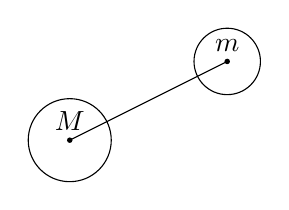
\begin{tikzpicture}
	\draw (0,0) circle [radius = 15pt] node[above] {$M$}
	(2,1) circle [radius=12pt] node[above] {$m$};
	\fill (0,0) circle[radius=1pt]
	(2,1) circle[radius=1pt];
	\draw (0,0) -- (2,1);

\end{tikzpicture}

\end{document}

  \caption{质量分别为$M,m$的星体}\label{fig:planet}
\end{figure}

\begin{example}
  两者皆可看作质点.
  若两星体由于引力而逐渐沿中心连线相互靠近,
  我们以$M$为参考系, 视作不动.
  当两者距离由$H$ 变化到 $h \, (H>h)$时, 引力做了多少功?

  我们知道, 当二者相距$x$时, 有
  \[
    F = \frac{GMm}{x^2}
  .\]

  \begin{figure}[ht]
    \centering
      \documentclass[border=3pt]{standalone}
\usepackage{tikz}
\usepackage{amsmath}
\usepackage{amssymb}
\usepackage{ctex}
\usetikzlibrary{matrix, calc, positioning}
\usepackage{pgfplots}
\pgfplotsset{compat=1.18}

\begin{document}

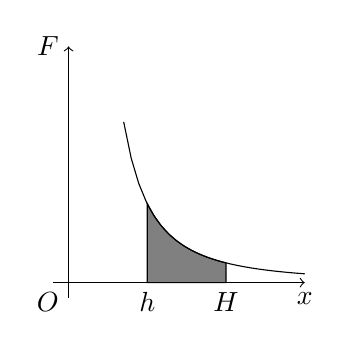
\begin{tikzpicture}
	\draw[->](-0.2,0)--(3,0)node[below]{$x$};
	\draw[->](0,-0.2)--(0,3)node[left]{$F$};
	\node[below left]at(0,0){$O$};
	\draw[fill=gray,domain=1:2] (1,0) -- plot({\x},{1/(\x)^2}) -- (2,0) -- cycle;
	\draw[domain=0.7:3] plot({\x}, {1/(\x)^2});
	\node[below]at(1,0){$h$};
	\node[below]at(2,0){$H$};
\end{tikzpicture}

\end{document}

    \caption{$F$-$x$图像}\label{fig:Fx}
  \end{figure}

  如\cref{fig:Fx}, 显然有$W_{Hh}$为阴影部分面积.
  \begin{align*}
    W_{Hh} & = \int _{h} ^{H} \frac{GMm}{x^2} \dif x    \\
    & = GMm \left(\frac{1}{h}-\frac{1}{H}\right)
  \end{align*}

  \paragraph{引力势能}
  实际上,任意保守场都具有一个势能函数,
  我们将无穷远处的引力势能视为$0$,
  则某点的重力势能等于物体从无穷远点运动到该点时,引力所做的功。即
  \[
    E_{\mathrm{p}} = \int_r^\infty \frac {GMm} {x^2} \dif x=\frac {GMm}r
  .\]

  对于两点电荷之间的电场力同理.

\end{example}
